\documentclass[crop]{standalone}

\usepackage{tikz}
\usetikzlibrary{positioning, arrows.meta, calc}

\begin{document}
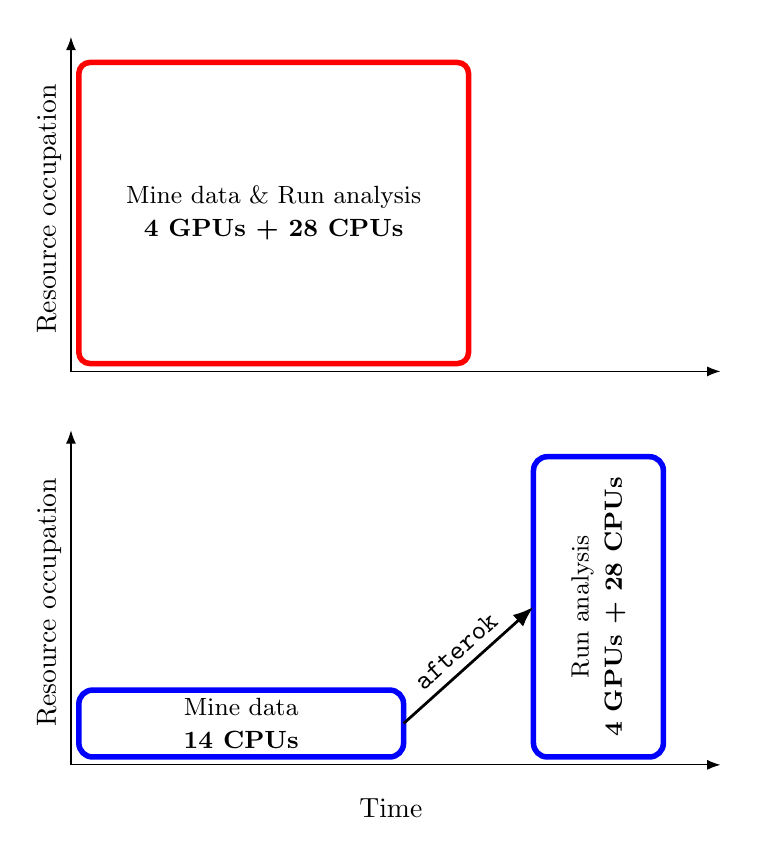
\begin{tikzpicture}[
  axis/.style = {->, >=Latex}
]
  % Place the plot axes
  \node[] (orig_0) {};
  \node[] (x_0) [right=8cm of orig_0] {};
  \node[] (y_0) [above=4cm of orig_0] {};

  \node[] (orig_1) [above=0.5cm of y_0] {};
  \node[] (x_1) [right=8cm of orig_1] {};
  \node[] (y_1) [above=4cm of orig_1] {};

  % Draw the axes
  \path[draw]
    (x_0)
      -- (orig_0.center)  node [midway,below,yshift=-0.3cm] {Time}
      -- (y_0) node [midway,above,sloped] {Resource occupation}
    (orig_0.center) edge[axis] (x_0.center)
    (orig_0.center) edge[axis] (y_0.center)
  ;
  \path[draw]
    (x_1)
      -- (orig_1.center)
      -- (y_1)  node [midway,above,sloped] {Resource occupation}
    (orig_1.center) edge[axis] (x_1.center)
    (orig_1.center) edge[axis] (y_1.center)
  ;

  \path[draw=red, line width=2pt, rounded corners=4pt]
    let
      \p{X_1} = ($(orig_1)!0.6!(x_1)+(0.1,0.1)$),
      \p{Y_1} = ($(orig_1)!0.9!(y_1)+(0.1,0.1)$),
      \p{orig_1} = ($(orig_1)+(0.1,0.1)$),
      \p{mid} = ($(\x{orig_1}, \y{orig_1})!0.5!(\x{Y_1}, \y{Y_1})$)
    in
      (\x{mid}, \y{mid})
        -- (\x{Y_1}, \y{Y_1})
        -- (\x{X_1}, \y{Y_1})
        -- (\x{X_1}, \y{X_1})
        -| cycle
      ($(\x{orig_1}, \y{orig_1})!0.5!(\x{X_1}, \y{Y_1})$) node[align=center] {\small Mine data \& Run analysis\\ \small \bfseries 4 GPUs + 28 CPUs}
  ;

  \path[draw=blue, line width=2pt, rounded corners=5pt]
    let
      \p{X_0} = ($(x_0)+(0.1,0.1)$),
      \p{Y_0} = ($(y_0)+(0.1,0.1)$),
      \p{orig_0} = ($(orig_0)+(0.1,0.1)$),
      \p{X_0_fetch} = ($(\x{orig_0}, \y{orig_0})!0.5!(\x{X_0}, \y{X_0})$),
      \p{Y_0_fetch} = ($(\x{orig_0}, \y{orig_0})!0.2!(\x{Y_0}, \y{Y_0})$),
      \p{orig_0_compute} = ($(\x{orig_0}, \y{orig_0})!0.7!(\x{X_0}, \y{X_0})$),
      \p{X_0_compute} = ($(\x{orig_0}, \y{orig_0})!0.9!(\x{X_0}, \y{X_0})$),
      \p{Y_0_compute} = (\x{orig_0_compute},0.9*\y{Y_0}),
      \p{mid_fetch} = ($(\x{orig_0}, \y{orig_0})!0.5!(\x{Y_0_fetch}, \y{Y_0_fetch})$),
      \p{mid_compute} = ($(\x{orig_0_compute}, \y{orig_0_compute})!0.5!(\x{Y_0_compute}, \y{Y_0_compute})$)
    in
      (\x{mid_fetch}, \y{mid_fetch})
        -- (\x{Y_0_fetch}, \y{Y_0_fetch})
        -- (\x{X_0_fetch}, \y{Y_0_fetch})
        -- (\x{X_0_fetch}, \y{X_0_fetch}) node [midway] (fetch_end) {}
        -| cycle
      (\x{mid_compute}, \y{mid_compute}) node [] (compute_begin) {}
        -- (\x{Y_0_compute}, \y{Y_0_compute})
        -- (\x{X_0_compute}, \y{Y_0_compute})
        -- (\x{X_0_compute}, \y{X_0_compute})
        -| cycle
      ($(\x{orig_0_compute}, \y{orig_0_compute})!0.5!(\x{X_0_compute}, \y{Y_0_compute})$) node[align=center,rotate=90] {\small Run analysis\\ \small \bfseries 4 GPUs + 28 CPUs}
      ($(\x{orig_0}, \y{orig_0})!0.5!(\x{X_0_fetch}, \y{Y_0_fetch})$) node[align=center] {\small Mine data\\ \small \bfseries 14 CPUs}
  ;

  \path[draw, line width=1pt, ->, >=Latex]
    (fetch_end.center) -- (compute_begin.center) node [midway,above,sloped] {\texttt{afterok}}
  ;
\end{tikzpicture}
\end{document}
